\documentclass[aspectratio=169]{beamer}
\usepackage{amsmath}
\usepackage{amssymb}
\usepackage{graphicx}
\usepackage{tcolorbox}
\usepackage{booktabs}
\usepackage{colortbl}
\usepackage{xcolor}
\usepackage{tikz}
\usetikzlibrary{shapes,arrows,positioning}

% Custom colors
\definecolor{primary}{RGB}{41, 128, 185}
\definecolor{secondary}{RGB}{52, 152, 219}
\definecolor{accent}{RGB}{231, 76, 60}
\definecolor{lightgray}{RGB}{236, 240, 241}

% Theme customization
\usetheme{Madrid}
\usecolortheme{whale}
\setbeamercolor{structure}{fg=primary}
\setbeamercolor{background canvas}{bg=white}
\setbeamercolor{normal text}{fg=black}

% Title page info
\title{Pre-Calculus 11}
\subtitle{Prerequisite Skills Review - Lesson 1.2}
\author{Created by Yi-Chen Lin}
\date{\today}

\begin{document}

\begin{frame}
    \titlepage
    \begin{tikzpicture}[remember picture,overlay]
        \fill[primary,opacity=0.1] (current page.south west) rectangle (current page.north east);
    \end{tikzpicture}
\end{frame}

% I) COMBINING LIKE-TERMS
\begin{frame}{Combining Like-Terms}
    \begin{tcolorbox}[colback=lightgray,colframe=primary,title=Definition]
        \footnotesize
        \begin{itemize}
            \item You can only add or subtract two terms if they are like-terms.
            \item \textbf{Like-terms:} Two algebraic terms that have the same variables and the exponents of the corresponding variables are the same.
            \item If they are not like-terms, then you cannot add or subtract them.
        \end{itemize}
    \end{tcolorbox}
\end{frame}

\begin{frame}{Combining Like-Terms - Practice}
    \begin{tcolorbox}[colback=lightgray,colframe=primary,title=Practice Problems]
        \footnotesize
        Indicate which of the following terms are like-terms. If they are like-terms, combine them:
        \begin{enumerate}
            \setlength{\itemsep}{0.5em}
            \item $3x$ and $x^3$
            \item $x^2y^2$ and $-5x^2y^3$
            \item $10a^2 - 4a$
            \item $5y + 12y^2 + 10y - 3y^2$
            \item $4a^2 - 3ab + 6b^2 - 8a^2 + 15ab + 2b^2$
        \end{enumerate}
    \end{tcolorbox}
\end{frame}

\begin{frame}{Combining Like-Terms - Solutions Part 1}
    \begin{tcolorbox}[colback=lightgray,colframe=accent,title=Detailed Solutions]
        \footnotesize
        \begin{enumerate}
            \setlength{\itemsep}{0.5em}
            \item $3x$ and $x^3$
            \quad \textbf{Solution:} Not Like-terms because the exponents for "x" are different.
            
            \item $x^2y^2$ and $-5x^2y^3$
            \quad \textbf{Solution:} Not Like-terms because they don't have the same variables (exponents for y are different).
            
            \item $10a^2 - 4a$
            \quad \textbf{Solution:} Not Like-terms (cannot be combined).
        \end{enumerate}
    \end{tcolorbox}
\end{frame}

\begin{frame}{Combining Like-Terms - Solutions Part 2}
    \begin{tcolorbox}[colback=lightgray,colframe=accent,title=Detailed Solutions]
        \footnotesize
        \begin{enumerate}
            \setcounter{enumi}{3}
            \setlength{\itemsep}{0.5em}
            \item $5y + 12y^2 + 10y - 3y^2$
            \quad \textbf{Solution:}
            \begin{itemize}
                \item Identify like-terms: $5y$ and $10y$ are like-terms, $12y^2$ and $-3y^2$ are also like-terms.
                \item Combine: $(5y + 10y) + (12y^2 - 3y^2) = 15y + 9y^2$
            \end{itemize}
            
            \item $4a^2 - 3ab + 6b^2 - 8a^2 + 15ab + 2b^2$
            \quad \textbf{Solution:}
            \begin{itemize}
                \item Identify like-terms: $4a^2$ and $-8a^2$; $-3ab$ and $15ab$; $6b^2$ and $2b^2$.
                \item Combine: $(4a^2 - 8a^2) + (-3ab + 15ab) + (6b^2 + 2b^2) = -4a^2 + 12ab + 8b^2$
            \end{itemize}
        \end{enumerate}
    \end{tcolorbox}
\end{frame}

% II) DO YOU REMEMBER HOW TO FOIL?
\begin{frame}{FOIL/Expansion - Multiplying Binomials}
    \begin{tcolorbox}[colback=lightgray,colframe=primary,title=Multiplying Binomials]
        \scriptsize
        \begin{itemize}
            \setlength{\itemsep}{0pt}
            \item When multiplying two binomials, you can visualize it as finding the area of a rectangle.
            \item \textbf{Example: } $(x+4)(x+5)$
            \vspace*{0.5em}
            \begin{center}
            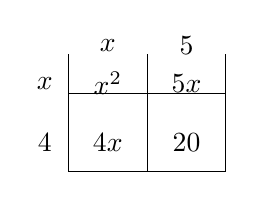
\begin{tikzpicture}
            \draw (0,0) grid (2,1.5);
            % Top labels
            \node at (0.5,1.6) {$x$};
            \node at (1.5,1.6) {$5$};
            % Left labels
            \node at (-0.3,1.125) {$x$};
            \node at (-0.3,0.375) {$4$};
            % Cell contents
            \node at (0.5,1.125) {$x^2$};
            \node at (1.5,1.125) {$5x$};
            \node at (0.5,0.375) {$4x$};
            \node at (1.5,0.375) {$20$};
            \end{tikzpicture}
            \end{center}
            \vspace*{-0.7em}
            \item The area is $x^2 + 5x + 4x + 20 = x^2 + 9x + 20$.
        \end{itemize}
    \end{tcolorbox}
\end{frame}

\begin{frame}{FOIL/Expansion - Another Method: FOIL}
    \begin{tcolorbox}[colback=lightgray,colframe=primary,title=Another Method: FOIL]
        \scriptsize
        \begin{itemize}
            \setlength{\itemsep}{0pt}
            \item \textbf{F}irst: Multiply the first terms of each binomial.
            \item \textbf{O}utside: Multiply the outer terms.
            \item \textbf{I}nside: Multiply the inner terms.
            \item \textbf{L}ast: Multiply the last terms of each binomial.
            \item \textbf{Example: } $(x+4)(x+5) = \underbrace{x \cdot x}_{F} + \underbrace{x \cdot 5}_{O} + \underbrace{4 \cdot x}_{I} + \underbrace{4 \cdot 5}_{L} = x^2 + 5x + 4x + 20 = x^2 + 9x + 20$.
        \end{itemize}
    \end{tcolorbox}
\end{frame}

\begin{frame}{Expand Binomials - Practice}
    \begin{tcolorbox}[colback=lightgray,colframe=primary,title=Practice Problems]
        \footnotesize
        Expand the Binomials:
        \begin{enumerate}
            \setlength{\itemsep}{0.5em}
            \item $(x - 5)(x - 2)$
            \item $(2x - 3)(5x - 8)$
            \item $(5x + 4)(7x - 6) - (8x - 2)(x + 3)$
        \end{enumerate}
    \end{tcolorbox}
\end{frame}

\begin{frame}{Expand Binomials - Solutions Part 1}
    \begin{tcolorbox}[colback=lightgray,colframe=accent,title=Detailed Solutions]
        \footnotesize
        \begin{enumerate}
            \setlength{\itemsep}{0.5em}
            \item $(x - 5)(x - 2)$
            \quad \textbf{Solution:}
            \begin{align*}
                (x - 5)(x - 2) &= x(x) + x(-2) + (-5)(x) + (-5)(-2) \\
                &= x^2 - 2x - 5x + 10 \\
                &= x^2 - 7x + 10
            \end{align*}
            \item $(2x - 3)(5x - 8)$
            \quad \textbf{Solution:}
            \begin{align*}
                (2x - 3)(5x - 8) &= 2x(5x) + 2x(-8) + (-3)(5x) + (-3)(-8) \\
                &= 10x^2 - 16x - 15x + 24 \\
                &= 10x^2 - 31x + 24
            \end{align*}
        \end{enumerate}
    \end{tcolorbox}
\end{frame}

\begin{frame}{Expand Binomials - Solutions Part 2}
    \begin{tcolorbox}[colback=lightgray,colframe=accent,title=Detailed Solutions]
        \footnotesize
        \begin{enumerate}
            \setcounter{enumi}{2}
            \setlength{\itemsep}{0.5em}
            \item $(5x + 4)(7x - 6) - (8x - 2)(x + 3)$
            \quad \textbf{Solution:}
            \begin{align*}
                & (5x + 4)(7x - 6) - (8x - 2)(x + 3) \\
                &= (35x^2 - 30x + 28x - 24) - (8x^2 + 24x - 2x - 6) \\
                &= (35x^2 - 2x - 24) - (8x^2 + 22x - 6) \\
                &= 35x^2 - 2x - 24 - 8x^2 - 22x + 6 \\
                &= (35x^2 - 8x^2) + (-2x - 22x) + (-24 + 6) \\
                &= 27x^2 - 24x - 18
            \end{align*}
        \end{enumerate}
    \end{tcolorbox}
\end{frame}

% III) Area and Perimeter with Expressions
\begin{frame}{Area and Perimeter - Practice}
    \begin{tcolorbox}[colback=lightgray,colframe=primary,title=Practice Problem]
        \footnotesize
        Given the dimensions of the solid, find an algebraic expression for the area and PERIMETER!!:
        
        \begin{center}
        \begin{tikzpicture}
        \draw (0,0) rectangle (4,2);
        \node at (2,-0.3) {$2x + 3y$};
        \node at (-0.5,1) {$x - 5$};
        \end{tikzpicture}
        \end{center}
        
        \begin{itemize}
            \item Area = ?
            \item Perimeter = ?
        \end{itemize}
    \end{tcolorbox}
\end{frame}

\begin{frame}{Area and Perimeter - Solutions}
    \begin{tcolorbox}[colback=lightgray,colframe=accent,title=Detailed Solutions]
        \footnotesize
        \begin{itemize}
            \item \textbf{Area:}
            \begin{align*}
                \text{Area} &= (x - 5)(2x + 3y) \\
                &= x(2x) + x(3y) + (-5)(2x) + (-5)(3y) \\
                &= 2x^2 + 3xy - 10x - 15y
            \end{align*}
            \item \textbf{Perimeter:}
            \begin{align*}
                \text{Perimeter} &= 2(x - 5) + 2(2x + 3y) \\
                &= 2x - 10 + 4x + 6y \\
                &= (2x + 4x) + 6y - 10 \\
                &= 6x + 6y - 10
            \end{align*}
        \end{itemize}
    \end{tcolorbox}
\end{frame}

% IV) BASIC FACTORING: GCF
\begin{frame}{Basic Factoring: GCF}
    \begin{tcolorbox}[colback=lightgray,colframe=primary,title=Introduction]
        \footnotesize
        \begin{itemize}
            \item Factoring is the opposite of expanding.
            \item When factoring, you are dividing out the greatest common factor (GCF) between several terms.
        \end{itemize}
    \end{tcolorbox}
\end{frame}

\begin{frame}{Basic Factoring: GCF - Practice 1}
    \begin{tcolorbox}[colback=lightgray,colframe=primary,title=Practice Problems]
        \footnotesize
        First indicate the GCF and then Factor out the GCF for each of the following:
        \begin{enumerate}
            \setlength{\itemsep}{0.5em}
            \item $20x^3 + 8xy$
            \item $21x^3y^2 + 35xy + 42y^4$
        \end{enumerate}
    \end{tcolorbox}
\end{frame}

\begin{frame}{Basic Factoring: GCF - Solutions 1}
    \begin{tcolorbox}[colback=lightgray,colframe=accent,title=Detailed Solutions]
        \footnotesize
        \begin{enumerate}
            \setlength{\itemsep}{0.5em}
            \item $20x^3 + 8xy$
            \quad \textbf{Solution:}
            \begin{itemize}
                \item Both terms are multiples of 4.
                \item Both terms have one $x$ variable.
                \item GCF = $4x$
                \item Factored: $4x(5x^2 + 2y)$
            \end{itemize}
            \item $21x^3y^2 + 35xy + 42y^4$
            \quad \textbf{Solution:}
            \begin{itemize}
                \item All three terms are multiples of 7.
                \item All three terms have a "y" variable.
                \item GCF = $7y$
                \item Factored: $7y(3x^3y + 5x + 6y^3)$
            \end{itemize}
        \end{enumerate}
    \end{tcolorbox}
\end{frame}

\begin{frame}{Basic Factoring: GCF - Practice 2}
    \begin{tcolorbox}[colback=lightgray,colframe=primary,title=Practice Problems]
        \footnotesize
        Find the Greatest common factor and then factor out the GCF for each of the following:
        \begin{enumerate}
            \setlength{\itemsep}{0.5em}
            \item $50x^4y^3 + 30x^6y^4$
            \item $90a^4b^7 + 25ab^6 + 65a^2b^5$
            \item $30(y - x) + 40x(y - x)$
            \item $28(x + y)^4 - 63(x + y)^3$
        \end{enumerate}
    \end{tcolorbox}
\end{frame}

\begin{frame}{Basic Factoring: GCF - Solutions 2 Part 1}
    \begin{tcolorbox}[colback=lightgray,colframe=accent,title=Detailed Solutions]
        \footnotesize
        \begin{enumerate}
            \setlength{\itemsep}{0.5em}
            \item $50x^4y^3 + 30x^6y^4$
            \quad \textbf{Solution:}
            \begin{itemize}
                \item GCF = $10x^4y^3$
                \item Factored: $10x^4y^3(5 + 3x^2y)$
            \end{itemize}
            \item $90a^4b^7 + 25ab^6 + 65a^2b^5$
            \quad \textbf{Solution:}
            \begin{itemize}
                \item GCF = $5ab^5$
                \item Factored: $5ab^5(18a^3b^2 + 5b + 13a)$
            \end{itemize}
        \end{enumerate}
    \end{tcolorbox}
\end{frame}

\begin{frame}{Basic Factoring: GCF - Solutions 2 Part 2}
    \begin{tcolorbox}[colback=lightgray,colframe=accent,title=Detailed Solutions]
        \footnotesize
        \begin{enumerate}
            \setcounter{enumi}{2}
            \setlength{\itemsep}{0.5em}
            \item $30(y - x) + 40x(y - x)$
            \quad \textbf{Solution:}
            \begin{itemize}
                \item GCF = $(y - x)$
                \item Factored: $(y - x)(30 + 40x) = 10(y - x)(3 + 4x)$
            \end{itemize}
            \item $28(x + y)^4 - 63(x + y)^3$
            \quad \textbf{Solution:}
            \begin{itemize}
                \item GCF = $7(x + y)^3$
                \item Factored: $7(x + y)^3(4(x + y) - 9) = 7(x + y)^3(4x + 4y - 9)$
            \end{itemize}
        \end{enumerate}
    \end{tcolorbox}
\end{frame}

% V) FACTORING DIFFERENCE OF SQUARES:
\begin{frame}{Factoring Difference of Squares: Conjugates}
    \begin{tcolorbox}[colback=lightgray,colframe=primary,title=Conjugates]
        \footnotesize
        Two binomials are conjugates if they have the same terms but a different sign in between them:
        \begin{itemize}
            \item Example: $x + 5 \rightarrow x - 5$
            \item Example: $7x - 10 \rightarrow 7x + 10$
            \item Example: $9a - 20 \rightarrow 9a + 20$
        \end{itemize}
    \end{tcolorbox}
\end{frame}

\begin{frame}{Difference of Squares: Multiplication Property}
    \begin{tcolorbox}[colback=lightgray,colframe=primary,title=What happens when you multiply a binomial with its conjugate?]
        \footnotesize
        \begin{enumerate}
            \item $(x + 5)(x - 5)$
            \quad \textbf{Solution:}
            \begin{align*}
                (x + 5)(x - 5) &= x^2 - 5x + 5x - 25 \\
                &= x^2 - 25
            \end{align*}
            \item $(7x - 10)(7x + 10)$
            \quad \textbf{Solution:}
            \begin{align*}
                (7x - 10)(7x + 10) &= 49x^2 + 70x - 70x - 100 \\
                &= 49x^2 - 100
            \end{align*}
        \end{enumerate}
        \vspace{0.5em}
        \begin{itemize}
            \item The middle two terms will always cancel each other out.
            \item The first and last terms are always perfect squares.
            \item The middle sign is always a subtraction.
        \end{itemize}
    \end{tcolorbox}
\end{frame}

\begin{frame}{Difference of Squares: Missing Terms}
    \begin{tcolorbox}[colback=lightgray,colframe=primary,title=Indicate the Missing Terms]
        \footnotesize
        \begin{enumerate}
            \setlength{\itemsep}{0.5em}
            \item $(x - 7)(x + 7) = x^2 - \rule{1cm}{0.15mm}$
            \item $(15a - 9b)(15a + 9b) = 225a^2 - \rule{1cm}{0.15mm}$
            \item $144x^2y^2 - 169 = (\rule{1cm}{0.15mm} - \rule{1cm}{0.15mm})(\rule{1cm}{0.15mm} + \rule{1cm}{0.15mm})$
            \item $49p^2q^2 - 25q^2 = (\rule{1cm}{0.15mm} - \rule{1cm}{0.15mm})(\rule{1cm}{0.15mm} + \rule{1cm}{0.15mm})$
            \item $9y^4 - 100 = (\rule{1cm}{0.15mm} - \rule{1cm}{0.15mm})(\rule{1cm}{0.15mm} + \rule{1cm}{0.15mm})$
        \end{enumerate}
    \end{tcolorbox}
\end{frame}

\begin{frame}{Difference of Squares: Missing Terms - Solutions}
    \begin{tcolorbox}[colback=lightgray,colframe=accent,title=Detailed Solutions]
        \footnotesize
        \begin{enumerate}
            \setlength{\itemsep}{0.5em}
            \item $(x - 7)(x + 7) = x^2 - \underline{49}$
            \item $(15a - 9b)(15a + 9b) = 225a^2 - \underline{81b^2}$
            \item $144x^2y^2 - 169 = (\underline{12xy} - \underline{13})(\underline{12xy} + \underline{13})$
            \item $49p^2q^2 - 25q^2 = (\underline{7pq} - \underline{5q})(\underline{7pq} + \underline{5q})$
            \item $9y^4 - 100 = (\underline{3y^2} - \underline{10})(\underline{3y^2} + \underline{10})$
        \end{enumerate}
    \end{tcolorbox}
\end{frame}

\begin{frame}{Factoring Difference of Squares: Rule}
    \begin{tcolorbox}[colback=lightgray,colframe=primary,title=Rule]
        \footnotesize
        \begin{itemize}
            \item When you have two perfect squares subtracting each other, you can factor it to a product of two conjugate binomials:
            \quad $a^2 - b^2 = (a - b)(a + b)$
            \item If the two perfect squares have a common factor, you can factor out the common factor first and then separate it as a product of conjugate binomials.
        \end{itemize}
    \end{tcolorbox}
\end{frame}

\begin{frame}{Factor Completely - Practice}
    \begin{tcolorbox}[colback=lightgray,colframe=primary,title=Practice Problems]
        \footnotesize
        FACTOR COMPLETELY:
        \begin{enumerate}
            \setlength{\itemsep}{0.5em}
            \item $144x^2y^2 - 49$
            \item $27a^2b^2 - 75$
            \item $49p^2q^5 - 81q$
            \item $16z^4 - 1$
        \end{enumerate}
    \end{tcolorbox}
\end{frame}

\begin{frame}{Factor Completely - Solutions Part 1}
    \begin{tcolorbox}[colback=lightgray,colframe=accent,title=Detailed Solutions]
        \footnotesize
        \begin{enumerate}
            \setlength{\itemsep}{0.5em}
            \item $144x^2y^2 - 49$
            \quad \textbf{Solution:}
            \begin{align*}
                144x^2y^2 - 49 &= (12xy)^2 - (7)^2 \\
                &= (12xy - 7)(12xy + 7)
            \end{align*}
            \item $27a^2b^2 - 75$
            \quad \textbf{Solution:}
            \begin{align*}
                27a^2b^2 - 75 &= 3(9a^2b^2 - 25) \\
                &= 3((3ab)^2 - (5)^2) \\
                &= 3(3ab - 5)(3ab + 5)
            \end{align*}
        \end{enumerate}
    \end{tcolorbox}
\end{frame}

\begin{frame}{Factor Completely - Solutions Part 2}
    \begin{tcolorbox}[colback=lightgray,colframe=accent,title=Detailed Solutions]
        \footnotesize
        \begin{enumerate}
            \setcounter{enumi}{2}
            \setlength{\itemsep}{0.5em}
            \item $49p^2q^5 - 81q$
            \quad \textbf{Solution:}
            \begin{align*}
                49p^2q^5 - 81q &= q(49p^2q^4 - 81) \\
                &= q((7pq^2)^2 - (9)^2) \\
                &= q(7pq^2 - 9)(7pq^2 + 9)
            \end{align*}
            \item $16z^4 - 1$
            \quad \textbf{Solution:}
            \begin{align*}
                16z^4 - 1 &= (4z^2)^2 - (1)^2 \\
                &= (4z^2 - 1)(4z^2 + 1) \\
                &= ((2z)^2 - (1)^2)(4z^2 + 1) \\
                &= (2z - 1)(2z + 1)(4z^2 + 1)
            \end{align*}
        \end{enumerate}
    \end{tcolorbox}
\end{frame}

\begin{frame}{Summary}
    \begin{tcolorbox}[colback=lightgray,colframe=primary,title=Key Concepts]
        \footnotesize
        \begin{itemize}
            \item Combining Like-Terms
            \item Expanding Polynomials (FOIL/Box Method)
            \item Basic Factoring (Greatest Common Factor - GCF)
            \item Factoring Difference of Squares
        \end{itemize}
    \end{tcolorbox}
\end{frame}

\end{document} 